\documentclass[xcolor={dvipsnames,table},aspectratio=169]{beamer}
\usepackage[utf8]{inputenc}
\usepackage[T1]{fontenc}
\usepackage[brazil]{babel}
\usepackage{graphics,amssymb,amsfonts,amsmath}
\usepackage{tikz}
\usepackage{enumerate,hyperref}
\usepackage{palatino}
\usepackage{ragged2e}
\usepackage{minted}
\usepackage{booktabs}
\usepackage{verbatim}
\usepackage[export]{adjustbox}
\usepackage{tikz}                   
\usepackage{xcolor}
\usepackage{textcomp} % para usar \textdegree
\usetikzlibrary{shadows}
\usetheme{AnnArbor}
\usecolortheme{orchid}
\usefonttheme[onlymath]{serif}

\newminted{java}{bgcolor=cyan!10}

\newcolumntype{C}[1]{>{\centering\let\newline\\\arraybackslash\hspace{0pt}}m{#1}}

\AtBeginSection[]{
  \begin{frame}
  \vfill
  \centering
  \begin{beamercolorbox}[sep=8pt,center,shadow=true,rounded=true]{title}
    \usebeamerfont{title}\insertsectionhead\par%
  \end{beamercolorbox}
  \vfill
  \end{frame}
}

\title[\sc{Gráficos em Java (Tópico Especial)}]{Gráficos em Java (Tópico Especial)}
\author[Roland Teodorowitsch]{Roland Teodorowitsch}
\institute[FPROG - EP - PUCRS]{Fundamentos de Programação - Escola Politécnica - PUCRS}
\date{24 de agosto de 2022}

\begin{document}
\justifying

%-------------------------------------------------------
\begin{frame}
	\titlepage
\end{frame}

%=======================================================
\section{Introdução}

%-------------------------------------------------------
\begin{frame}\frametitle{Objetivos}
\begin{itemize}
	\item Criar programas em Java que utilizam formas geométricas básicas
	\item Ter um programa com uma estrutura simples a partir da qual se possa desenhar algumas formas geométricas
	\item NÃO se pretende aprofundar a discussão sobre as classes usadas para criar e controlar janelas em uma \emph{Graphic User Interface} (GUI)
\end{itemize}
\end{frame}

%-------------------------------------------------------
\begin{frame}\frametitle{Em \texttt{main}}
\begin{itemize}
	\item Inicia-se criando um objeto chamado \texttt{frame} da classe \texttt{JFrame}
	\item Um \texttt{JFrame} corresponde a uma moldura dentro da qual se podem colocar ou desenhar outros componentes (no exemplo a seguir, a moldura ou janela será de 400 por 400 \emph{pixels})
	\item Para este \emph{frame}, define-se então o tamanho (chamada ao método \texttt{setSize}) e a operação de fechamento padrão (chamada ao método \texttt{setDefaultCloseOperation})
	\item Em seguida cria-se um componente (\texttt{JComponent}), definindo para este componente um método para desenhar a janela (basicamente este método, que se chama \texttt{paintComponent}, chama o método \texttt{draw}, que será responsável por desenhar a janela)
	\item Adiciona-se o componente ao \emph{frame} (chamada de método \texttt{add})
	\item E, por fim, torna-se o frame \emph{visível} (chamada de método \texttt{setVisible})
\end{itemize}
\end{frame}

%-------------------------------------------------------
\begin{frame}\frametitle{No método \texttt{draw}}
\begin{itemize}
	\item É este método que efetivamente desenha as figuras geométricas na janela (e deve ser declarado como \texttt{static} para poder ser chamado a partir de \texttt{main})
	\item O método \texttt{draw} tem como parâmetro um objeto da classe \texttt{Graphics}
	\item A classe \texttt{Graphics} possui uma série de métodos com os quais se pode desenhar diferentes figuras geométricas (retângulos, elipses, segmentos de reta, etc.)
	\item Pode-se considerar que os objetos da classe \texttt{Graphics} funcionam de forma semelhante a \texttt{System.out}, porém desenhando figuras em um \emph{frame} e não textos em um terminal
	\item No exemplo a seguir, o método \texttt{setColor} define a cor padrão de impressão como sendo azul, e \texttt{fillRect} é usado para desenhar duas fileiras com quadrados preenchidos de forma alternada
	\end{itemize}
\end{frame}

%=======================================================
\section{Exemplo}

%-------------------------------------------------------
\begin{frame}\frametitle{Exemplo}
\begin{itemize}
	\item O exemplo a seguir desenha duas fileiras de retângulos alternados em uma janela
\begin{figure}[h]	
	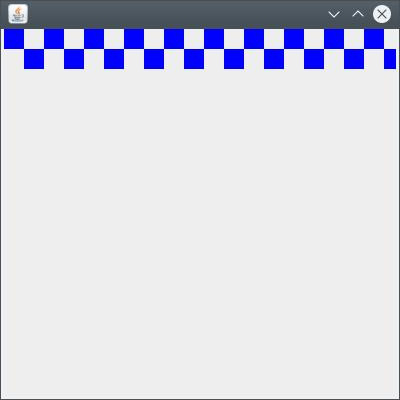
\includegraphics[height=0.6\paperheight,center]{pucrs-ep-fprog-unidade_04-graficos_em_java-laminas-exemplo.jpg}
\end{figure}
\end{itemize}
\end{frame}

%-------------------------------------------------------
\begin{frame}[fragile]\frametitle{\texttt{TwoRowsOfSquares.java} {\tiny (HORSTMANN, 2013, p. 180-181)}}
{\tiny
\begin{javacode}
import java.awt.Color;
import java.awt.Graphics;
import javax.swing.JFrame;
import javax.swing.JComponent;

/** This program draws two rows of squares. */
public class TwoRowsOfSquares {

   public static void draw(Graphics g) {
      final int width = 20;
      g.setColor(Color.BLUE);
      // Top row. Note that the top left corner of the drawing has coordinates (0, 0)
      int x = 0;
      int y = 0;
      for (int i = 0; i < 10; i++) {
         g.fillRect(x, y, width, width);
         x = x + 2 * width;
      }
      // Second row, offset from the first one
      x = width;
      y = width;
      for (int i = 0; i < 10; i++) {
         g.fillRect(x, y, width, width);
         x = x + 2 * width;
      }
   }
\end{javacode}
}
\end{frame}

%-------------------------------------------------------
\begin{frame}[fragile]\frametitle{\texttt{TwoRowsOfSquares.java} {\tiny (HORSTMANN, 2013, p. 180-181)}}
{\tiny
\begin{javacode}
   public static void main(String[] args) {
      // Do not look at the code in the main method
      // Your code will go into the draw method above
      JFrame frame = new JFrame();
      final int FRAME_WIDTH = 400;
      final int FRAME_HEIGHT = 400;
      frame.setSize(FRAME_WIDTH, FRAME_HEIGHT);
      frame.setDefaultCloseOperation(JFrame.EXIT_ON_CLOSE);
      JComponent component = new JComponent() {
         public void paintComponent(Graphics graph) {
            draw(graph);
         }
      };
      frame.add(component);
      frame.setVisible(true);
   }
}
\end{javacode}
}
\end{frame}

%=======================================================
\section{Alguns métodos de \texttt{Graphics}}

%-------------------------------------------------------
\begin{frame}[fragile]\frametitle{Alguns métodos de \texttt{Graphics} (1)}
{\scriptsize
\begin{center}
  \begin{tabular}{|p{6cm}|p{3cm}|p{4cm}|}
\hline
    \textbf{Método} & \textbf{Resultado} & \textbf{Explicação} \\
\hline
\texttt{g.drawRect(x, y, width, height)}
&
\begin{figure}[h]
	
\includegraphics[height=0.1\paperheight,center]{pucrs-ep-fprog-unidade_04-graficos_em_java-laminas-retangulo.png}
\end{figure}
& \texttt{(x, y)} é o canto superior esquerdo.\\
\hline
\texttt{g.drawOval(x, y, width, height)}
&
\begin{figure}[h]
	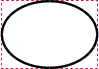
\includegraphics[height=0.1\paperheight,center]{pucrs-ep-fprog-unidade_04-graficos_em_java-laminas-elipse.png}
\end{figure}
& \texttt{(x, y)} é o canto superior esquerdo do retângulo que limita a elipse. Para desenhar um cículo usa-se o mesmo valor para \texttt{width} e \texttt{height}.\\
\hline
\texttt{g.fillRect(x, y, width, height)}
&
\begin{figure}[h]
	
\includegraphics[height=0.1\paperheight,center]{pucrs-ep-fprog-unidade_04-graficos_em_java-laminas-retangulo_preenchido.png}
\end{figure}
& O retângulo é desenhado preenchido.\\
\hline
  \end{tabular}
\end{center}
}
\end{frame}

%-------------------------------------------------------
\begin{frame}[fragile]\frametitle{Alguns métodos de \texttt{Graphics} (2)}
{\scriptsize
\begin{center}
  \begin{tabular}{|p{6cm}|p{3cm}|p{4cm}|}
\hline
    \textbf{Método} & \textbf{Resultado} & \textbf{Explicação} \\
\hline
\texttt{g.fillOval(x, y, width, height)}
&
\begin{figure}[h]
	
\includegraphics[height=0.1\paperheight,center]{pucrs-ep-fprog-unidade_04-graficos_em_java-laminas-elipse_preenchida.png}
\end{figure}
& A elipse é desenhada preenchida.\\
\hline
\texttt{g.drawLine(x1, y1, x2, y2)}
&
\begin{figure}[h]
	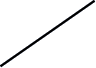
\includegraphics[height=0.1\paperheight,center]{pucrs-ep-fprog-unidade_04-graficos_em_java-laminas-reta.png}
\end{figure}
& \texttt{(x1, y1)} e \texttt{(x2, y2)} são os pontos inicial e final de um segmento de reta.\\
\hline
\texttt{g.drawString("Message", x, y)}
&
\begin{figure}[h]
	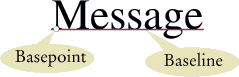
\includegraphics[height=0.1\paperheight,center]{pucrs-ep-fprog-unidade_04-graficos_em_java-laminas-message.png}
\end{figure}
	& \texttt{(x, y)} é o ponto base (\emph{basepoint}).\\
\hline
  \end{tabular}
\end{center}
}
\end{frame}

%-------------------------------------------------------
\begin{frame}[fragile]\frametitle{Alguns métodos de \texttt{Graphics} (3)}
{\scriptsize
\begin{center}
  \begin{tabular}{|p{6cm}|p{3cm}|p{4cm}|}
\hline
    \textbf{Método} & \textbf{Resultado} & \textbf{Explicação} \\
\hline
\texttt{g.setColor(color)}
&
A partir deste ponto, os métodos para desenhar ou desenhar preenchido usarão a cor selecionada.
& Use \texttt{Color.RED}, \texttt{Color.GREEN}, \texttt{Color.BLUE} e assim por diante.\\
\hline
  \end{tabular}
\end{center}
}
\end{frame}

%=======================================================
\section{Exercícios}

%-------------------------------------------------------
\begin{frame}\frametitle{Exercícios}
\begin{enumerate}

	\item Escreva uma aplicação gráfica em Java para desenhar a seguinte face:
	\begin{figure}[h]
		
\includegraphics[height=2cm,center]{pucrs-ep-fprog-unidade_04-graficos_em_java-laminas-exercicio_1.png}
	\end{figure}
	{\tiny Fonte: Horstmann (2013, p. 197)}

	\item Escreva uma aplicação gráfica em Java para desenhar uma espiral retangular como a mostrada na figura a seguir:
	\begin{figure}[h]
		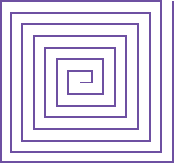
\includegraphics[height=2cm,center]{pucrs-ep-fprog-unidade_04-graficos_em_java-laminas-exercicio_2.png}
	\end{figure}
	{\tiny Fonte: Horstmann (2013, p. 197)}
\end{enumerate}
\end{frame}

%=======================================================
\section{Referências}

%-------------------------------------------------------
\begin{frame}\frametitle{Referências}
\noindent{HORSTMANN, C. \textbf{Java for Everyone – Late Objetct}. 2. ed. Hoboken: Wiley, 2013. xxxiv, 589 p.}
\end{frame}

%=======================================================
\end{document}

